\documentclass[aspectratio=169,11pt]{beamer}
\usepackage{fathomnet-course}
% generated by write_numbers.py from results/reference_results.json - do not edit
\newcommand{\RefCrops}{23{,}664}
\newcommand{\RefDives}{1{,}465}
\newcommand{\RefTopTenDives}{21\,\%}
\newcommand{\RefTwoTrain}{444}
\newcommand{\RefTwoTest}{148}
\newcommand{\RefThr}{0.05}
\newcommand{\RefThrTrain}{98.4\,\%}
\newcommand{\RefThrTest}{98.0\,\%}
\newcommand{\RefCSPhylumMajority}{30.4\,\%}
\newcommand{\RefCSPhylumCentroid}{26.4\,\%}
\newcommand{\RefCSPhylumKnn}{55.0\,\%}
\newcommand{\RefCSPhylumTree}{50.3\,\%}
\newcommand{\RefCSLabelMajority}{1.3\,\%}
\newcommand{\RefCSLabelCentroid}{15.9\,\%}
\newcommand{\RefCSLabelKnn}{33.6\,\%}
\newcommand{\RefCSLabelTree}{23.7\,\%}
\newcommand{\RefCSLabelBest}{33.6\,\%}
\newcommand{\RefZooBestName}{neural network (MLP)}
\newcommand{\RefZooBest}{64.6\,\%}
\newcommand{\RefZooBestPixels}{46.3\,\%}
\newcommand{\RefZooBestColour}{48.4\,\%}
\newcommand{\RefZooRows}{majority baseline & 1.3\,\% & 1.3\,\% & $<$1\,s \\
nearest centroid & 39.9\,\% & 37.9\,\% & 2\,s \\
5-nearest neighbours & 69.9\,\% & 53.4\,\% & $<$1\,s \\
decision tree & 100.0\,\% & 20.5\,\% & 48\,s \\
random forest & 100.0\,\% & 56.1\,\% & 93\,s \\
logistic regression & 90.7\,\% & 63.7\,\% & 21\,s \\
neural network (MLP) & 92.4\,\% & 64.6\,\% & 13\,s \\}
\newcommand{\RefRandomAcc}{63.5\,\%}
\newcommand{\RefRandomAccKnn}{53.5\,\%}
\newcommand{\RefTrainLogregRandom}{90.7\,\%}
\newcommand{\RefTrainKnnRandom}{70.0\,\%}
\newcommand{\RefImageAcc}{57.5\,\%}
\newcommand{\RefImageAccKnn}{45.5\,\%}
\newcommand{\RefTrainLogregImage}{91.1\,\%}
\newcommand{\RefTrainKnnImage}{71.0\,\%}
\newcommand{\RefDiveAcc}{49.6\,\%}
\newcommand{\RefDiveAccKnn}{35.5\,\%}
\newcommand{\RefTrainLogregDive}{91.0\,\%}
\newcommand{\RefTrainKnnDive}{71.6\,\%}
\newcommand{\RefSeenDiveRandom}{97\,\%}
\newcommand{\RefRecallRows}{species & 33 & 67\,\% \\
genus & 21 & 69\,\% \\
family & 8 & 64\,\% \\
order & 6 & 56\,\% \\
class & 6 & 44\,\% \\
phylum & 1 & 27\,\% \\
other rank & 4 & 58\,\% \\}
\newcommand{\RefSevKingdom}{55\,\%}
\newcommand{\RefSevNear}{21\,\%}
\newcommand{\RefRandPhylumAcc}{80.0\,\%}
\newcommand{\RefDivePhylumAcc}{72.6\,\%}
\newcommand{\RefDiveFone}{0.475}
\newcommand{\RefDiveAccSingle}{49.8\,\%}

\title{How a computer sees an animal}
\subtitle{\coursetitle\\[2pt]\small Session 3 -- features, CNNs and the classifier zoo}
\date{}
\author{}
\begin{document}
\maketitle

\begin{frame}{Last time: the characters were the problem}
\begin{columns}[c]
\column{0.5\textwidth}
With 30 colour characters, the best simple classifier labelled \RefCSLabelBest\ of the test crops correctly (79 labels).\\[6pt]
A taxonomist does not identify a sea star by its \emph{average colour}, but by
\begin{itemize}\small
  \item body plan (arms, disc, symmetry)
  \item texture (spines, plates, polyps)
  \item shape of parts (tentacles, fins)
\end{itemize}
\column{0.45\textwidth}
\begin{block}{Today's question}
Can a computer find such characters \emph{by itself}?
\end{block}
\end{columns}
\end{frame}

\begin{frame}{A picture is a table of numbers}
\centering
\begin{tikzpicture}[>=Stealth]
  \foreach \x in {0,...,7} \foreach \y in {0,...,5} {
    \pgfmathsetmacro{\v}{mod(37*\x+53*\y+11*\x*\y,100)}
    \fill[coral!\v!sea!40] (\x*0.45,\y*0.45) rectangle ++(0.45,0.45);
  }
  \draw[ocean] (0,0) rectangle (3.6,2.7);
  \node[below, font=\small] at (1.8,-0.05) {$224\times224$ pixels $\times$ 3 colours};
  \draw[->, thick] (4,1.35) -- (5.2,1.35);
  \node[align=left, font=\small, anchor=west, text width=6.2cm] at (5.4,1.35) {150{,}528 numbers between 0 and 255\\[2pt]
     \muted{(we shrink the crop to $16\times16\times3 = 768$ numbers: the feature set \texttt{pixels})}};
\end{tikzpicture}
\vspace{10pt}
\begin{alertblock}{Why raw pixels are poor characters}
The same sea star, shifted by a few pixels, rotated, or filmed in other light, gives completely different numbers.
Pixel number 3{,}417 means ``something orange at this spot'' -- not ``has five arms''.
\end{alertblock}
\end{frame}

\begin{frame}{Three feature sets}
\small
\begin{tabularx}{\linewidth}{@{}l r X X@{}}
\toprule
\textbf{feature set} & \textbf{numbers} & \textbf{what they are} & \textbf{biology analogy} \\
\midrule
\texttt{pixels} & 768 & the crop at $16\times16$ & a blurry thumbnail \\
\texttt{colour\_stats} & 30 & mean colour, brightness, redness, contrast, edge strength, hue \& brightness histograms & characters a field biologist could measure with a colour chart \\
\texttt{cnn} & 512 & what a convolutional neural network pre-trained on 1.2 million everyday photos responds to & characters learned from looking at a huge number of things \\
\bottomrule
\end{tabularx}
\end{frame}

\begin{frame}{Convolutional neural networks (CNN) in one slide}
\centering
\begin{tikzpicture}[>=Stealth, font=\small,
  lay/.style={draw=ocean, fill=sea!12, minimum height=19mm, align=center, text width=22mm}]
  \node[lay, fill=white] (in) {crop\\[2pt]\tiny $224\times224\times3$};
  \node[lay, right=5mm of in] (l1) {\textbf{early layers}\\[2pt]\footnotesize edges, colour blobs};
  \node[lay, right=6mm of l1] (l2) {\textbf{middle layers}\\[2pt]\footnotesize textures: spines, polyps};
  \node[lay, right=6mm of l2] (l3) {\textbf{late layers}\\[2pt]\footnotesize parts: arms, tentacles, eyes};
  \node[lay, right=6mm of l3, fill=coral!15, draw=coral] (emb) {\textbf{embedding}\\[2pt]\footnotesize 512 numbers};
  \foreach \a/\b in {in/l1, l1/l2, l2/l3, l3/emb} \draw[->, thick] (\a) -- (\b);
  \draw[decorate, decoration={brace, amplitude=5pt, mirror}] ([yshift=-2mm]l1.south west) -- ([yshift=-2mm]l3.south east)
      node[midway, below=5pt, text width=110mm, align=center, font=\footnotesize] {each layer = many small \textbf{filters} that slide over the image, learned from ImageNet (dogs, cars, mushrooms \dots)};
\end{tikzpicture}
\vspace{2pt}
\begin{itemize}\footnotesize
  \item We use \textbf{ResNet-18} (11 million learned numbers) and keep the 512 numbers before its last layer.
  \item We do \textbf{not} train the CNN: it is a ready-made character extractor. This is called \hl{transfer learning}.
  \item Why does ImageNet help for deep-sea animals? Edges, textures and shapes are the same everywhere.
\end{itemize}
\end{frame}

\begin{frame}{A map of 3,000 crops in each feature space}
\centering
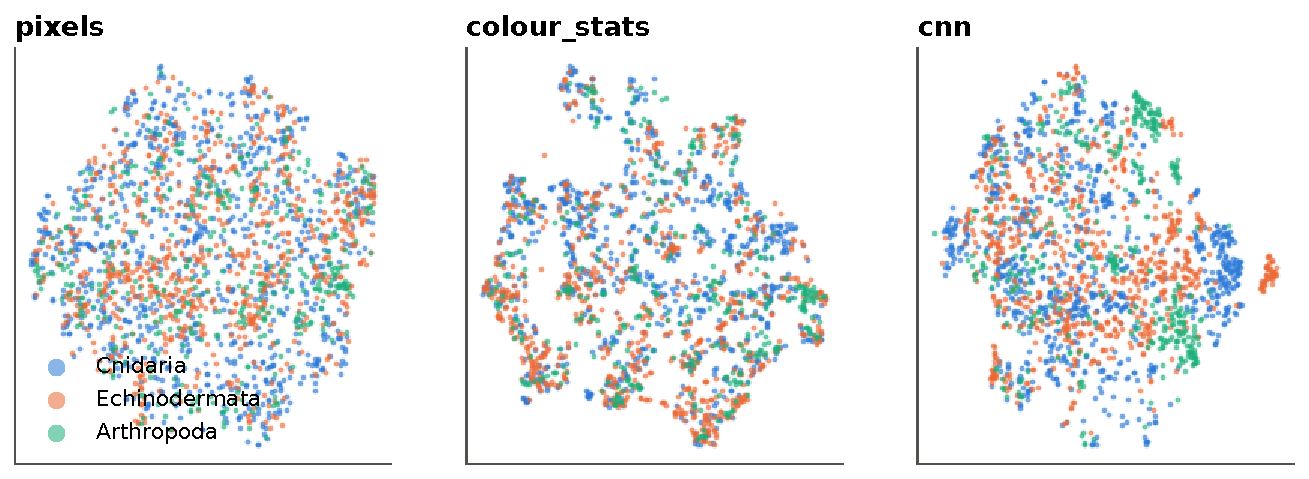
\includegraphics[width=\linewidth]{figures/tsne_maps.pdf}\\[2pt]
\small Each space drawn as a 2-D map (t-SNE: crops that are similar in the feature space stay close), coloured by phylum.
With CNN features, \hl{islands of a single phylum} appear -- although the CNN was never told what a phylum is. Much still overlaps.
\end{frame}

\begin{frame}{The classifier zoo: 7 classifiers $\times$ 3 feature sets}
\begin{columns}[c]
\column{0.52\textwidth}
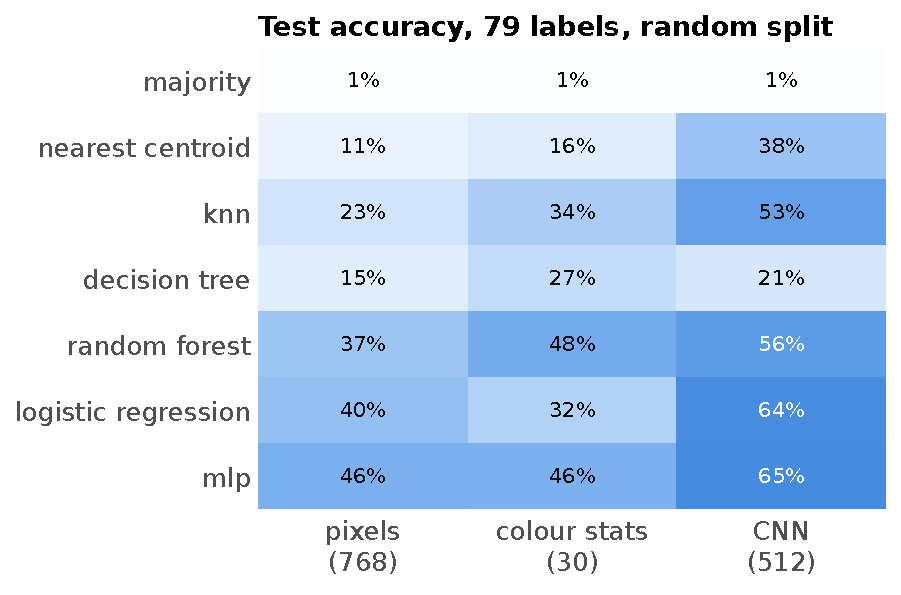
\includegraphics[width=\linewidth]{figures/zoo_heatmap.pdf}
\column{0.45\textwidth}
\small
\begin{itemize}
  \item Same data, same split, 79 labels.
  \item Best: \hl{\RefZooBestName} on CNN features: \RefZooBest.
  \item Best on pixels: \RefZooBestPixels; on colour stats: \RefZooBestColour.
  \item The \emph{column} (features) matters much more than the \emph{row} (classifier).
\end{itemize}
\vspace{4pt}
\muted{\scriptsize random 75/25 split of all \RefCrops\ crops; reference run, numbers will differ slightly in your notebook}
\end{columns}
\end{frame}

\begin{frame}{Training accuracy vs. test accuracy (CNN features)}
\small
\centering
\begin{tabular}{@{}lrrr@{}}
\toprule
classifier & train & test & fit time \\
\midrule
\RefZooRows
\bottomrule
\end{tabular}

\vspace{6pt}
\raggedright
The single tree and the random forest are perfect on the training crops -- they \emph{memorise}.
The forest still does reasonably on new crops; the single tree does not. \hl{Only the test column counts.}
\end{frame}

\begin{frame}{Lab 2 -- features and the zoo}
\task{
\begin{enumerate}
  \item Look at a crop as numbers (16 $\times$ 16 pixels).
  \item Compute the three feature sets (CNN: $\approx$15 min on a 4-core laptop, a few minutes on a Colab GPU).
  \item Compare the maps. Which space groups the phyla?
  \item Nearest neighbours: which crops look ``most similar'' in each space?
  \item Run the zoo; answer: \emph{features or classifier -- which matters more?}
  \item How well are the labels of \emph{your group} recognised?
\end{enumerate}}
\end{frame}
\end{document}
